% A magyarázó agent belső felépítése (5. fejezet). Fordítás: pdflatex magyarazo.tex
\documentclass[tikz,border=4pt]{standalone}
\usepackage[utf8]{inputenc}
\usepackage[T1]{fontenc}
\usepackage{times}
\usetikzlibrary{positioning,arrows.meta,shapes.geometric}
\definecolor{det}{HTML}{1D294D}
\definecolor{detbg}{HTML}{E6ECF7}
\definecolor{llm}{HTML}{B7791F}
\definecolor{llmbg}{HTML}{FEEFCF}
\begin{document}
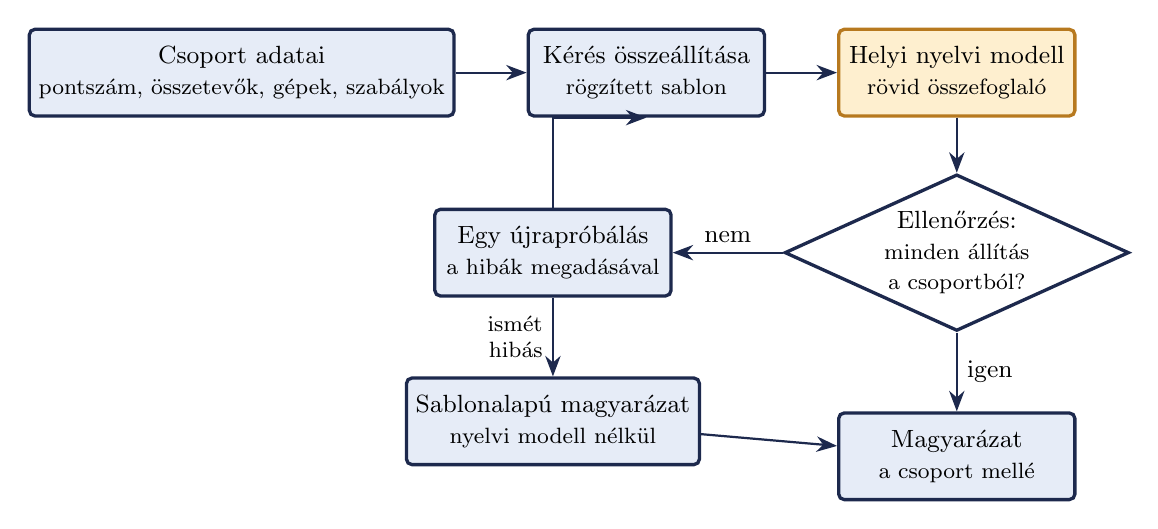
\begin{tikzpicture}[
  font=\small, node distance=7mm and 9mm,
  lepes/.style={draw=det, fill=detbg, very thick, rounded corners=2pt, minimum width=30mm,
               minimum height=11mm, align=center},
  llmlepes/.style={lepes, draw=llm, fill=llmbg},
  dec/.style={diamond, aspect=2.2, draw=det, fill=white, very thick, align=center, inner sep=1pt},
  flow/.style={-{Stealth[length=2.6mm]}, thick, draw=det},
]
\node[lepes] (in) {Csoport adatai\\\footnotesize pontszám, összetevők, gépek, szabályok};
\node[lepes, right=of in] (prompt) {Kérés összeállítása\\\footnotesize rögzített sablon};
\node[llmlepes, right=of prompt] (llm) {Helyi nyelvi modell\\\footnotesize rövid összefoglaló};
\node[dec, below=of llm] (chk) {Ellenőrzés:\\\footnotesize minden állítás\\\footnotesize a csoportból?};
\node[lepes, below=10mm of chk] (ok) {Magyarázat\\\footnotesize a csoport mellé};
\node[lepes, left=14mm of chk] (retry) {Egy újrapróbálás\\\footnotesize a hibák megadásával};
\node[lepes, below=10mm of retry] (fb) {Sablonalapú magyarázat\\\footnotesize nyelvi modell nélkül};
\draw[flow] (in) -- (prompt);
\draw[flow] (prompt) -- (llm);
\draw[flow] (llm) -- (chk);
\draw[flow] (chk) -- node[right]{igen} (ok);
\draw[flow] (chk) -- node[above]{nem} (retry);
\draw[flow] (retry) |- (prompt.south);
\draw[flow] (retry) -- node[left, align=right, font=\footnotesize]{ismét\\ hibás} (fb);
\draw[flow] (fb) -- (ok);
\end{tikzpicture}
\end{document}
